\chapter{Recursively Defined Domains}

Chapter 10 of Tennent's book

\section{Motivation}

\begin{enumcirc}
	%
	\item
	%
	One reason that we studied category theory is to understand a general principle
	behind the construction of recursively defined domains, such as the following
	$\Omega$ that you encountered before:
	%
	\begin{align*}
		\Omega       & \simeq \prths{\hat{\Sigma} + \Z \times \Omega + \prths{\Z \to \Omega}}_\bot \\
		\hat{\Sigma} & \defeq \Sigma \cup \braces{\abort} \times \Sigma \simeq \Sigma + \Sigma     \\
	\end{align*}
	%
	\item
	%
	If we write the RHS of the above isomorphism as $F\prths{\Omega}$, the formula
	says:
	%
	\[
		\Omega \simeq F\prths{\Omega}
	\]
	%
	That is, $\Omega$ is a fixed point of $F$.
	%
	In fact, $\Omega$ is not just a fixed point, but the best fixed point where
	``the best'' means something very similar to ``the least'' in the standard
	fixed point theorem of the domain theory.
	%
	\item
	%
	We will generalize the standard least fixed point theorem of the domain theory
	and obtain a general categorical least fixed point theorem.
	%
	This generalization closely follows the intuition that categories are
	generalized partially ordered sets (and functors are generalized monotone
	functions).
	%
	Then, we will instantiate our generalization with a particular category
	constructed out of domains and a particular kind of continuous functions called
	embeddings.
	%
\end{enumcirc}

\section{$\omega$-chain and co-limit of $\omega$-chain}

\begin{enumcirc}
	%
	\item
	%
	Let's start by remembering ingredients that we needed when expressing the
	standard least fixed point theorem of the domain theory.
	%
	\begin{enumrm}
		%
		\item
		%
		A partially ordered set $D$ has the least element.
		%
		\item
		%
		Every chain in $D$ has the last upper bound
		%
		\item
		%
		A function $f$ on $D$ is continuous (i.e., monotone and
		chain-limit-preserving).
		%
	\end{enumrm}
	%
	Then, the theorem says that $f$ has the least fixed point $x_0$.
	%
	That is, $f\prths{x_0} = x_0$ and for all $y$ s.t. $f\prths{y} = y$, $x_0 \leq
		y$.\footnote{property that is a bit stronger than $x_0$ being the least fixed
		point}
	%
	\item
	%
	In the categorical generalization of the theorem,
	%
	\begin{enumrm}
		%
		\item
		%
		$D$ becomes a category $\Cc$;
		%
		\item
		%
		$f \in \brackets{D \to D}$ becomes a functor $F : \Cc \to \Cc$;
		%
		\item
		%
		$x_0$ becomes an object in $\Cc$;
		%
		\item
		%
		the least element of $D$ becomes the initial object of $\Cc$;
		%
	\end{enumrm}
	%
	Note that \ul{the monotonicity of $f$} \footnote{preservation of the
		$\sqsubseteq$ relation} translates to $F$'s morphism map being type-checked
	with respect to its object map.
	%
	(i.e., for all $g: x \to y$, $F\prths{g}: F\prths{x} \to F\prths{y}$)
	%
	This translated property is a part of the conditions for $F$ being a functor.
	%
	Thus, the monotonicity already holds for $F$ in a sense.
	%
	\item
	%
	Ok, what remain?
	%
	We still need to generalize
	%
	\begin{enumrm}
		%
		\item
		%
		chains
		%
		\item
		%
		least upper bounds (or limiets) of chains
		%
		\item
		%
		limit-preservation
		%
	\end{enumrm}
	%
	\item
	%
	A \ul{$\omega$-chain} in a category $\Cc$ is a countably infinite sequence of
	objects $\prths{x_0, x_1, x_2, \ldots}$ of $\Cc$ and a collection of morphisms
	$\braces{f_i : x_i \to x_{i+1}}_{i \ge 0}$ in $\Cc$.
	%
	The best way to understand this is to imagine the following figure:
	%
	\[
		\begin{tikzcd}[row sep=large]
			x_0 \arrow[r, "f_0"] & x_1 \arrow[r, "f_1"] & x_2 \arrow[r, "f_2"] & \cdots
		\end{tikzcd}
	\]
	%
	We use $\triangle$ to denote a $\omega$-chain.
	%
	\item
	%
	A \ul{co-cone} of an $\omega$-chain $\triangle = \braces{\prths{x_i, f_i}}_{i
			\ge 0}$ is a pair of object $x$ and a collection of morphisms $\braces{g_i :
			x_i \to x}_{i \ge 0}$ such that for all $i \ge 0$, $g_{i+1} \circ f_i = g_i$,
	i.e., in picture,
	%
	\[
		\begin{tikzcd}[row sep=large]
			x_i \arrow[r, "f_i"] \arrow[dr, "g_i"'] & x_{i+1} \arrow[d, "g_{i+1}"] \\
			& x
		\end{tikzcd}
	\]
	%
	commutes.
	%
	\item
	%
	Intuitively, an $\omega$-chain is a generalized chain, and the object $x$ of a
	co-cone $\prths{x, \braces{g_i}_i}$ of $\triangle$ is a generalized upper bound
	of the chain.
	%
	Each $g_i: x_i \to x$ provides a way to view that $x$ is larger than or equal
	to $x_i$.
	%
	Meanwhile, each $f_i: x_i \to x_{i+1}$ provides a way to view that $x_{i+1}$ is
	larger than or equal to $x_i$.
	%
	The commutativity requirement says that these two views should be compatible.
	%
	\item
	%
	A \ul{co-cone} of an $\omega$-chain $\triangle = \braces{\prths{x_i, f_i}}_{i
			\ge 0}$ is \ul{co-limiting} if for every co-cone $\prths{x', \braces{g'_i}_i}$
	of $\triangle$, there exists a unique morphism $h: x \to x'$ such that for all
	$i$,
	%
	\[
		g'_i = h \circ g_i,
	\]
	%
	in a diagram,
	%
	\[
		\begin{tikzcd}[row sep=large]
			x_i \arrow[dr, "g_i"'] \arrow[ddr, swap, "g'_i", bend right = 30] & \\
			& x \arrow[d, dashed, "!h"] \\
			& x' \\
		\end{tikzcd}
	\]
	%
	Intuitively, the very existence of $h$ says that $x$ is smaller than or equal
	to $x'$.
	%
	The commutativity and the uniqueness say that $h$'s explanation about why $x$
	is smaller than or equal to $x'$ follows automatically and canonically from the
	$g_i$ and the $g'_i$.
	%
	\item
	%
	A co-limiting co-cone $\prths{x, \braces{g_i}_i}$ of an $\triangle$ is a
	generalization of the least upper bound of a chain.
	%
	I usually imagine the following visual image whenever I work with an
	$\omega$-chain, a co-cone, or a co-limiting co-cone:
	%
	\[
		\begin{tikzcd}[row sep=large]
			x_0 \arrow[r, "f_0"] \arrow[drrrr, "g_0", bend right = 20] \arrow[ddrrrr, "g'_0", bend right = 100] &
			x_1 \arrow[r, "f_1"] \arrow[drrr, "g_1", bend right = 20]  \arrow[ddrrr, "g'_1", bend right = 100]  &
			x_2 \arrow[r, "f_2"] \arrow[drr, "g_2", bend right = 20]   \arrow[ddrr, "g'_2", bend right = 100]   &
			x_3 \arrow[r, "f_3"] \arrow[dr, "g_3", bend right = 20]    \arrow[ddr, "g'_3", bend right = 100]    & \cdots \\
			& & & & x \arrow[d, dashed, "h"] \\
			& & & & x'
		\end{tikzcd}
	\]
	%
	\begin{exercisetab}
		%
		Construct co-limiting co-cones of $\omega$-chains in the category of Set.
		%
		Do the same thing in the poset (partially ordered set) category $\prths{2^\N,
				\subseteq}$ and in the category of predomains.
		%
	\end{exercisetab}
	%
\end{enumcirc}

\section{$\omega$-continuous functor}

\begin{enumcirc}
	%
	\item
	%
	Let $\Cc$ and $\Dc$ be categories that have {co-limiting co-cones}\footnote{in
		other words, co-limits} for all $\omega$-chains.
	%
	We will call such categories as \ul{chain-complete categories}.
	%
	\item
	%
	A functor $F: \Cc \to \Dc$ is \ul{$\omega$-continuous} if it maps a co-limit of
	an $\omega$-chain to a co-limit of an $\omega$-chain, that is,
	%
	\begin{align*}
		\textrm{for every } \omega\textrm{-chain } & \triangle = \braces{\prths{x_i, f_i}}_{i \ge 0} \textrm{ in } \Cc,                               \\
		\textrm{for every co-limit }               & \prths{x, \braces{g_i}_i} \textrm{ of } \triangle,                                               \\
		                                           & \prths{F\prths{x}, \braces{F\prths{g_i}}_i} \textrm {is a co-limit of }                          \\
		                                           & F\prths{\triangle} = \prths{\braces{F\prths{x_i}}_i, \braces{F\prths{f_i}}_i} \textrm{ in } \Dc.
	\end{align*}
	%
	\item
	%
	Intuitively, this $\omega$-continuity of $F$ means that $F$ preserves the least
	upper bound of an increasing chain.
	%
	\item
	%
	Note that a functor $F$ always maps a co-cone of an $\omega$-chain to a co-cone
	of an $\omega$-chain: visually,
	%
	\[
		\qquad \quad
		\begin{tikzcd}[row sep=large]
			x_0 \arrow[r, "f_0"] \arrow[drr, "g_0", bend right = 30] &
			x_1 \arrow[r, "f_1"] \arrow[dr, "g_1", bend right = 30] &
			x_2 \arrow[r, "f_2"] \arrow[d, "g_2", bend right = 30] & \cdots \\
			& & x
		\end{tikzcd}
		\qquad \qquad
		\textrm{category } \Cc
	\]
	%
	\[
		\begin{tikzcd}
			F\prths{x_0} \arrow[r, "F\prths{f_0}"] \arrow[drr, "F\prths{g_0}", bend right = 30] &
			F\prths{x_1} \arrow[r, "F\prths{f_1}"] \arrow[dr, "F\prths{g_1}", bend right = 30] &
			F\prths{x_2} \arrow[r, "F\prths{f_2}"] \arrow[d, "F\prths{g_2}", bend right = 30] & \cdots \\
			& & F\prths{x}
		\end{tikzcd}
		\qquad
		\textrm{category } \Dc
	\]
	%
	If the diagram in $\Cc$ commutes, the diagram in $\Dc$ also commutes.
	%
	This is because the preservation of $\circ$ and $\id$ by a functor implies that
	the functor maps every commuting diagram to a commuting diagram.

	The situation is similar to the fact that a monotone function $f$ from a
	predomain to a predomain maps an upper bound of a chain to an upper bound of a
	chain.
	%
	\item
	%
	However, the functoriality of $F$ doesn't ensure that if $\prths{x,
			\braces{g_i}_i}$ is a co-limit of $\triangle$, so is $\prths{F\prths{x},
			\braces{F\prths{g'_i}}_i}$.

	When $F$ satisfies this additional property, we say that $F$ is
	$\omega$-continuous.
	%
	\begin{exercisetab}
		%
		Show that the functor from Set to Set
		%
		\begin{align*}
			F\prths{S} & = \Z \times S                                                   \\
			F\prths{f} & = \id_\Z \times f = \lambda \prths{n, s}. \prths{n, f\prths{s}}
		\end{align*}
		%
		is $\omega$-continuous.
		%
	\end{exercisetab}
	%
\end{enumcirc}

\section{Fixed point theorem}

\begin{theorem}
	%
	Let $\Cc$ be a category with an initial object $x_0$.
	%
	Assume that $\Cc$ is chain-complete (i.e., every $\omega$-chain $\triangle$ in
	$\Cc$ has a co-limit).
	%
	Then, for every $\omega$-continuous functor $F: \Cc \to \Cc$, there exists an
	object $\subsctext{x}{fix}$ in $\Cc$ and a morphism $\eta:
		F\prths{\subsctext{x}{fix}} \to \subsctext{x}{fix}$ such that
	%
	\begin{enumrm}
		%
		\item
		%
		$\eta$ is an isomorphism, i.e.,
		%
		$\exists$ a morphism $\psi : \subsctext{x}{fix} \to F\prths{\subsctext{x}{fix}}$ s.t.
		%
		$\eta \circ \psi = \id_{\subsctext{x}{fix}}$ and $\psi \circ \eta = \id_{F\prths{\subsctext{x}{fix}}}$;
		%
		\item
		%
		for every morphism $\eta': F\prths{y} \to y$, there exists a unique morphism
		$\rho: \subsctext{x}{fix} \to y$ such that
		%
		\[
			\begin{tikzcd}
				F\prths{\subsctext{x}{fix}} \arrow[r, "\eta"] \arrow[d, swap, "F\prths{\rho}"] & \subsctext{x}{fix} \arrow[d, dashed, "\rho"] \\
				F\prths{y} \arrow[r, "\eta'"] & y
			\end{tikzcd}
		\]
		%
	\end{enumrm}
	%
\end{theorem}
%
\begin{enumcirc}
	%
	\item
	%
	Intuitively, the theorem says that $subsctext{x}{fix}$ is the least fixed point
	of $F$.
	%
	The condition (i) says that $\subsctext{x}{fix}$ is a fixed point.
	%
	The condition (ii) says that it is the least fixed point.
	%
	\item
	%
	The proof is complex, but note that difficult.
	%
	Very similar to the proof of the standard fixed point theorem of the domain
	theory.
	%
	We will study only some parts of the proof.
	%
	\item
	%
	The key part of the proof is to construct $\subsctext{x}{fix}$.
	%
	Here we use the initial object $x_0$ of $\Cc$, the functoriality of $F$, and
	the chain completeness of $\Cc$
	%
	(They correspond to $\bot$, the monotonicity of a continuous function $f$ and the chain completeness of a predomain $D$
	in the proof of the fixed-point theorem in domain theory).

	We construct a chain:
	%
	\[
		\triangle \defeq
		\begin{tikzcd}[row sep=large]
			x_0 \arrow[r, "f_0"] & F\prths{x_0} \arrow[r, "f_1"] & F^2\prths{x_0} \arrow[r, "f_2"] & F^3\prths{x_0} \arrow[r, "f_3"] & \cdots
		\end{tikzcd}
	\]
	%
	where $f_0$ is a unique morphism from the initial object $x_0$ to
	$F\prths{x_0}$,
	%
	and $f_i = F^i\prths{f_0}$ is a unique morphism from $F^i\prths{x_0}$ to
	$F^{i+1}\prths{x_0}$.

	Since $\Cc$ is chain-complete, there exists a co-limit $\prths{x,
			\braces{g_i}}$ of the chain $\triangle$ that we just built.
	%
	\[
		\begin{tikzcd}[row sep=large]
			x_0 \arrow[r, "f_0"] \arrow[drrr, "g_0", bend right = 20]          &
			F\prths{x_0} \arrow[r, "F\prths{f_0}"] \arrow[drr, "g_1", bend right = 20]  &
			F^2\prths{x_0} \arrow[r, "F^2\prths{f_0}"] \arrow[dr, "g_2", bend right = 20] &
			F^3\prths{x_0} \arrow[r, "F^3\prths{f_0}"] \arrow[d, "g_3", bend right = 20]  & \cdots \\
			& & & \subsctext{x}{fix}  \\
		\end{tikzcd}
	\]
	%
	\item
	%
	Next we build $\eta: F\prths{\subsctext{x}{fix}} \to \subsctext{x}{fix}$.
	%
	Here we use the $\omega$-continuity of $F$.
	%
	Apply $F$ to the diagram.
	%
	This gives us
	%
	\[
		\begin{tikzcd}[row sep=large]
			\triangle' \defeq
			F\prths{x_0} \arrow[r, "F\prths{f_0}"] \arrow[drrr, "F\prths{g_0}", bend right = 20]          &
			F^2\prths{x_0} \arrow[r, "F^2\prths{f_0}"] \arrow[drr, "F\prths{g_1}", bend right = 20]  &
			F^3\prths{x_0} \arrow[r, "F^3\prths{f_0}"] \arrow[dr, "F\prths{g_2}", bend right = 20] &
			F^4\prths{x_0} \arrow[r, "F^4\prths{f_0}"] \arrow[d, "F\prths{g_3}", bend right = 20]  & \cdots \\
			& & & F\prths{\subsctext{x}{fix}}  \\
		\end{tikzcd}
		.
	\]
	%
	Since $F$ is $\omega$-continuous, this is a \ul{co-limiting} co-cone of the
	chain $\triangle'$, which is the $x_0$-truncated version of $\triangle$.
	%
	\item
	%
	Because $x_0$ is the initial object, we can add $x_0$ to the diagram and get a
	\ul{co-limiting} co-cone,
	%
	\[
		\begin{tikzcd}[row sep=large]
			x_0 \arrow[r, "f_0"] \arrow[drrrr, "g_0'", bend right = 30]          &
			F\prths{x_0} \arrow[r, "F\prths{f_0}"] \arrow[drrr, "F\prths{g_0}", bend right = 20]          &
			F^2\prths{x_0} \arrow[r, "F^2\prths{f_0}"] \arrow[drr, "F\prths{g_1}", bend right = 20]  &
			F^3\prths{x_0} \arrow[r, "F^3\prths{f_0}"] \arrow[dr, "F\prths{g_2}", bend right = 20] &
			F^4\prths{x_0} \arrow[r, "F^4\prths{f_0}"] \arrow[d, "F\prths{g_3}", bend right = 20]  & \cdots \\
			& & & & F\prths{\subsctext{x}{fix}}  \\
		\end{tikzcd}
	\]
	%
	where $g_0'$ is a unique morphism from $x_0$ to $F\prths{\subsctext{x}{fix}}$.
	%
	The leftmost triangle commutes because of the initiality of $x_0$.

	Now we have two co-limits, $\subsctext{x}{fix}$ and
	$F\prths{\subsctext{x}{fix}}$, of the same chain $\triangle$.
	%
	One general result (which is easy to show) is that two co-limits of a chain are
	isomorphic, which means in our case that there exist morphisms $\eta:
		F\prths{\subsctext{x}{fix}} \to \subsctext{x}{fix}$ and $\psi:
		\subsctext{x}{fix} \to F\prths{\subsctext{x}{fix}}$ such that
	%
	\[
		\psi \circ \eta = \id_{F\prths{\subsctext{x}{fix}}} \quad \textrm{ and } \quad \eta \circ \psi = \id_{\subsctext{x}{fix}}.
	\]
	%
	We just proved (i) of the theorem.
	%
	We leave the proof of (ii) as an exercise.
	%
	\item
	%
	Why is (ii) in the theorem useful?
	%
	Because it allows us to define a morphism from $\subsctext{x}{fix}$ to some
	$y$.
	%
\end{enumcirc}

\section{Famous example of the fixed point theorem}

\begin{enumcirc}
	%
	\item
	%
	One big motivation for developing domain theory was to find a solution of the
	following equation for space $D$:
	%
	\begin{equation} \label{eq:space}
		D \simeq D \to D.
	\end{equation}
	%
	Such a space is needed (as you will see later in the course) to define a
	mathematical or denotational semantics of the untyped lambda calculus, which
	forms the core of most functional programming languages.
	%
	\item
	%
	But note that if $D$ is a set and $D \to D$ is the set of all functions on $D$,
	the only solution of \cref{eq:space} is the singleton set (of course, in this
	case, $\simeq$ means some bijection between two sets).
	%
	This is because if $D$ contains more than one element, the cardinality of
	$\brackets{D \to D}$ is always strictly larger than that of $D$.
	%
	\item
	%
	Using domains, we can find a solution of \cref{eq:space} (using the fixed point
	theorem).
	%
	But we have to be careful about defining a category on which we apply the
	theorem.
	%
	\item
	%
	Here is the category $\Dom[EP]$ that we use.
	%
	\begin{enumrm}
		%
		\item
		%
		Objects of $\Dom[EP]$ are domains; i.e., partially ordered set where all chains
		have least upper bounds and the least element exists.
		%
		\item
		%
		Morphisms from a domain $D$ to a domain $D'$ are strict (i.e.
		$\bot$-preserving) continuous functions $f$ from $D$ to $D'$ such that there
		exists a continuous function $g: D' \to D$ with
		%
		\[
			g \circ f = \id_D \quad \textrm{ and } \quad f \circ g \sqsubseteq \id_{D'}.
		\]
		%
		\item
		%
		$\circ$ is the usual function composition.
		%
		\item
		%
		$\id_D$ is the identity function on $D$.
		%
	\end{enumrm}
	%
	\item
	%
	Compared with the category $\Dom$ of domains and continuous functions, this
	category $\Dom[EP]$ has a rather unusual notion of morphisms.
	%
	In $\Dom[EP]$, a morphism $f: D \to D'$ should be not just continuous, but also
	strict.
	%
	More importantly, it should have $g: D' \to D$ such that
	%
	\[
		g \circ f = \id_D \quad \textrm{ and } \quad f \circ g \sqsubseteq \id_{D'}.
	\]
	%
	In picture,
	%
	\[
		\begin{tikzcd}[sep=3em]
			D \arrow[r, "f"] \arrow[rd, "\id_{D}"'] & D' \arrow[d, "g"] \\
			& D
		\end{tikzcd}
		\quad \textrm{ and } \quad
		\begin{tikzcd}[column sep= 1.2em, row sep=1.3em]
			D' \arrow[rr, "g"] \arrow[rrdd, "\id_{D'}"'] & & D \arrow[dd, "f"] \\
			& \arrow[ur, phantom, "\sqsupseteq" marking] & \\
			& & D'
		\end{tikzcd}
	\]
	%
	Intuitively, the existence of such $g$ means that $D'$ is built by putting
	additional elements above existing elements of $D$, and $g$ maps all additional
	elements to their best under-approximations in $D$.
	%
	Here is some picture that shows this intuition.
	%
	\begin{center}
		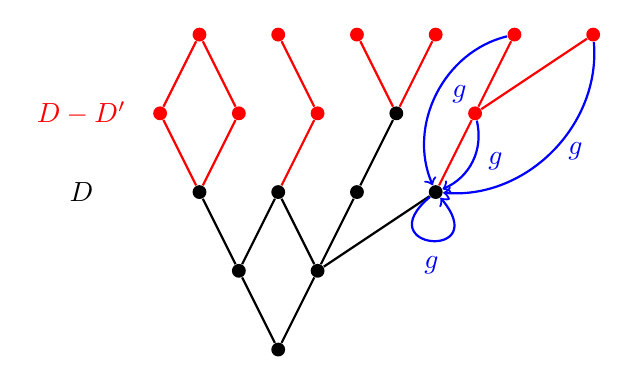
\begin{tikzpicture}
			% Define nodes
			\node[circle, fill=black, inner sep=0pt, minimum size=5pt] (b00) at (0,0) {};
			\node[circle, fill=black, inner sep=0pt, minimum size=5pt] (b10) at (-0.5,1) {};
			\node[circle, fill=black, inner sep=0pt, minimum size=5pt] (b11) at (0.5,1) {};
			\node[circle, fill=black, inner sep=0pt, minimum size=5pt] (b20) at (-1,2) {};
			\node[circle, fill=black, inner sep=0pt, minimum size=5pt] (b21) at (0,2) {};
			\node[circle, fill=black, inner sep=0pt, minimum size=5pt] (b22) at (1,2) {};
			\node[circle, fill=black, inner sep=0pt, minimum size=5pt] (b23) at (2,2) {};
			\node[circle, fill=black, inner sep=0pt, minimum size=5pt] (b30) at (1.5,3) {};

			\node[circle, fill=red, inner sep=0pt, minimum size=5pt] (r30) at (-1.5,3) {};
			\node[circle, fill=red, inner sep=0pt, minimum size=5pt] (r31) at (-0.5,3) {};
			\node[circle, fill=red, inner sep=0pt, minimum size=5pt] (r32) at (0.5,3) {};
			\node[circle, fill=red, inner sep=0pt, minimum size=5pt] (r33) at (2.5,3) {};
			\node[circle, fill=red, inner sep=0pt, minimum size=5pt] (r40) at (-1,4) {};
			\node[circle, fill=red, inner sep=0pt, minimum size=5pt] (r41) at (0,4) {};
			\node[circle, fill=red, inner sep=0pt, minimum size=5pt] (r42) at (1,4) {};
			\node[circle, fill=red, inner sep=0pt, minimum size=5pt] (r43) at (2,4) {};
			\node[circle, fill=red, inner sep=0pt, minimum size=5pt] (r44) at (3,4) {};
			\node[circle, fill=red, inner sep=0pt, minimum size=5pt] (r45) at (4,4) {};

			% Draw black solid edges
			\draw[thick] (b00) -- (b10);
			\draw[thick] (b00) -- (b11);
			\draw[thick] (b10) -- (b20);
			\draw[thick] (b10) -- (b21);
			\draw[thick] (b11) -- (b21);
			\draw[thick] (b11) -- (b22);
			\draw[thick] (b11) -- (b23);
			\draw[thick] (b22) -- (b30);

			% Draw red dashed edges
			\draw[thick, red] (b20) -- (r30);
			\draw[thick, red] (b20) -- (r31);
			\draw[thick, red] (b21) -- (r32);
			\draw[thick, red] (b23) -- (r33);
			\draw[thick, red] (r30) -- (r40);
			\draw[thick, red] (r31) -- (r40);
			\draw[thick, red] (r32) -- (r41);
			\draw[thick, red] (b30) -- (r42);
			\draw[thick, red] (b30) -- (r43);
			\draw[thick, red] (r33) -- (r44);
			\draw[thick, red] (r33) -- (r45);

			\node[color=red] (DD) at (-2.5,3) {$D-D'$};
			\node[] (D) at (-2.5,2) {$D$};

			\draw[->, bend left=40, color=blue, thick] (r33) to node[pos=0.5, right=0.2em] {$g$} (b23);
			\draw[->, bend left=50, color=blue, thick] (r45) to node[pos=0.5, right=0.2em] {$g$} (b23);
			\draw[->, bend right=50, color=blue, thick] (r44) to node[pos=0.5, right=0.2em] {$g$} (b23);
			\draw[->, color=blue, thick] (b23) to [out=220, in=310, looseness=20] node[pos=0.5, below=0.2em] {$g$} (b23);

		\end{tikzpicture}
	\end{center}
	%
	Where $D-D'$ is the set of additional elements in $D'$ and $g$ maps elements of
	$D'$ to their best under-approximations in $D$.
	%
	What this means is that a morphism $f: D \to D'$ is really saying that $D'$ is
	larger than $D$.
	%
	\item
	%
	A morphism $f: D \to D'$ in $\Dom[EP]$ is called \ul{embedding} and a
	corresponding $g: D' \to D$ is called \ul{projection}.

	If you happen to take a course on program analysis, this pair of embedding $f$
	and projection $g$ is closely related to the Galois connection there.

	Note That the definition doesn't say that there exists only one projection $g$
	for a given embedding $f$.
	%
	That is, there may be multiple projections.
	%
	But this doesn't happen.

	\begin{lemma}
		%
		For every embedding $f: D \to D'$, and projections $g_1, g_2: D' \to D$ for
		$f$, we have that
		%
		\[
			g_1 = g_2.
		\]
		%
	\end{lemma}
	%
	\begin{proof}
		%
		We will show that $g_1 \sqsubseteq g_2$.
		%
		A similar argument can show the opposite inequality.
		%
		\[
			g_1 = \id_D \circ g_1 =
			\prths{g_2 \circ f} \circ g_1 =
			g_2 \circ \prths{f \circ g_1} \sqsubseteq
			g_2 \circ \id_{D'} =
			g_2.
		\]
		%
	\end{proof}
	%
	We write $f^\textrm{P}$ to denote the unique projection for an embedding $f$.
	%
	\item
	%
	The category $\Dom[EP]$ has an initial object, which is a singleton domain
	$\prths{\braces{\bot}, \sqsubseteq}$\footnote{$x \sqsubseteq y$ iff $x = y$}.
	%
	It also has a co-limit for any $\omega$-chain.
	%
	We will not prove this.
	%
	But we point out one important property of these co-limits.

	\begin{lemma} \label{lem:co-limit}
		%
		Consider the following co-cone of an $\omega$-chain $\triangle$:
		%
		\[
			\triangle =
			\begin{tikzcd}[row sep=large]
				D_0 \arrow[r, "f_0"] \arrow[drr, "h_0", bend right = 30] &
				D_1 \arrow[r, "f_1"] \arrow[dr, "h_1", bend right = 30] &
				D_2 \arrow[r, "f_2"] \arrow[d, "h_2", bend right = 30] & \cdots \\
				& & D'
			\end{tikzcd}
		\]
		%
		Let $h_i^\textrm{P}$ be the projection for the embedding $h_i$.
		%
		Then, $D'$ is \ul{co-limiting} if and only if
		%
		\[
			\bigsqcup_{i=0}^\infty \prths{h_i \circ h_i^\textrm{P}} = \id_{D'}.
		\]
		%
		Note that $h_i \circ h_i^\textrm{P} \sqsubseteq \id_{D'}$.
		%
		We can easily show that $\braces{h_i \circ h_i^\textrm{P}}_{i \ge 0}$ is an
		increasing chain in $\brackets{D' \toc D'}$.
		%
		The condition says that the least upper bound of the chain is $\id_{D'}$.
		%
	\end{lemma}
	%
	This lemma says that \ul{the order on morphisms} plays an important role in
	deciding whether $D'$ is a co-limit or not.
	%
	One important consequence is the following lemma.
	%
	\begin{lemma} \label{lem:omega-cont}
		%
		A functor $F: \Dom[EP] \to \Dom[EP]$ is $\omega$-continuous if for every
		co-cone of an $\omega$-chain $\triangle$
		%
		\[
			\begin{tikzcd}[row sep=large]
				D_0 \arrow[r, "f_0"] \arrow[drr, "h_0", bend right = 30] &
				D_1 \arrow[r, "f_1"] \arrow[dr, "h_1", bend right = 30] &
				D_2 \arrow[r, "f_2"] \arrow[d, "h_2", bend right = 30] & \cdots \\
				& & D'
			\end{tikzcd}
			,
		\]
		%
		\[
			\bigsqcup_{i=0}^\infty \prths{h_i \circ h_i^\textrm{P}} = \id_{D'}
			\implies
			\bigsqcup_{i=0}^\infty \prths{F\prths{h_i} \circ F\prths{h_i^\textrm{P}}} = \id_{F\prths{D'}}.
		\]
		%
	\end{lemma}
	%
	\begin{proof}
		%
		This is a direct consequence of the previous lemma.
		%
	\end{proof}
	%
	\item
	%
	\cref{lem:omega-cont} is our tool to check the $\omega$-continuity of a functor $F$ on
	$\Dom[EP]$.
	%
	If this check passes, by the fixed point theorem, we know that there exists a
	domain $D$ such that
	%
	\[
		F\prths{D} \simeq D
	\]
	%
	\begin{enumrm}
		%
		\item
		%
		Our functor
		%
		$F\prths{\Omega} = \prths{\Sigma + \Sigma + \Z \times \Omega + \brackets{\Z \to \Omega}}_\bot$
		%
		is an example of such a functor.
		%
		\item
		%
		Another famous example is the following $G$ that defines the function space.

		$G\prths{D} = \brackets{D \toc D}$ \dots the domain of continuous functions in $D$.

		For every $f: D \to D'$,
		%
		\[
			G\prths{f}: G\prths{D} \to G\prths{D'} \textrm{ i.e., } \brackets{D \toc D} \to \brackets{D' \toc D'}
		\]
		%
		\[
			G\prths{f}\prths{h} = f \circ h \circ f^\textrm{P}\footnotemark.
		\]
		\footnoteeqn[0]{
			%
			We are using the projection of $f$ here.
			%
			If $f$ were just a continuous function, we couldn't do it.
			%
		}
		%
	\end{enumrm}
	%
	\begin{exercise}
		%
		Prove that $F$ and $G$ are indeed $\omega$-continuous.
		%
	\end{exercise}
	%
	\begin{exercise}
		%
		Prove \cref{lem:co-limit}.
		%
		(This is not easy)
		%
	\end{exercise}
	%
	If you are familiar with program analysis and abstract interpretation, you
	might have noticed that there we do something similar when defining the
	abstract domain for function space.
	%
	One thing to keep in mind is that in domain theory, $a \sqsubseteq b$ means
	that $b$ is more informative than $a$, while in program analysis, $a
		\sqsubseteq b$ means that $a$ is more informative than $b$.
	%
\end{enumcirc}
